Il voice over IP è un metodo per gestire le chiamate telefoniche su internet, invece che utilizzare la rete telefonica tradizionale. In questo modo, è possibile effettuare chiamate vocali utilizzando una connessione internet, invece di una linea telefonica dedicata.
La PTSN (Public Switched Telephone Network) è una rete a commutazione di circuito, mente le rete internet è a commutazione di pacchetto. La PTSN è progettata per gestire le chiamate vocali, mentre la rete internet è progettata per gestire una vasta gamma di dati, tra cui testo, immagini e video.
In VoIP, la voce viene trasmessa interamente in formato digitale (e pacchettizzata).
Nella rete PTSN la trasmissione analogica della voce avviene nell'ultimo miglio (POTS, plain old telephone service), mentre il resto è digitale.
Ci sono due tipi di operatori:
\begin{itemize}
	\item \textbf{Over the top (OTT)}: forniscono servizi VoIP senza possedere l'infrastruttura di rete sottostante. 
	\item \textbf{Network operator (Carrier-based)}: Operatori di rete che offrono servizi VoIP.
\end{itemize}
\section{Tipi di chiamate VoIP}
Diversi tipi di chiamate VoIP possono essere effettuate:
\begin{itemize}
	\item \textbf{VoIP-VoIP}
	\item \textbf{VoIP-PTSN/PTSN-VoIP}
	\item \textbf{VoIP-Mobile Radio Network/Mobile Radio Network-VoIP}
\end{itemize}
Nel secondo e terzo tipo deve essere garantita la possibilità di interconnessione tra le reti.
\subsection{VoIP-VoIP}
Si divide a sua volta in:
\begin{itemize}
	\item \textbf{VoIP puro}: la comunicazione avviene tra due terminai che supportano nativamente VoIP (ad esempio un pc o telefono VoIP).
	I pacchetti vocali vengono instradati usando internet sull'intero cammino, bypassando la rete PTSN.
	\begin{figure}[H]
		\centering
		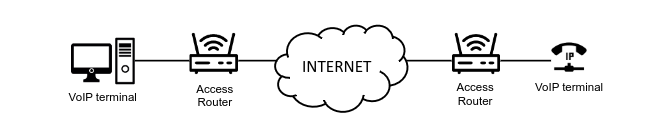
\includegraphics[width=0.8\textwidth]{pictures/6/pureVoip.png}
	\end{figure}
	\item \textbf{Terminali adattati}: La comunicazione avviene tramite terminali PTSN che sono stati adattati a utilizzare VoIP. I pacchetti vengono instradati usando internet, bypassando la rete PTSN.
	\begin{figure}[H]
		\centering
		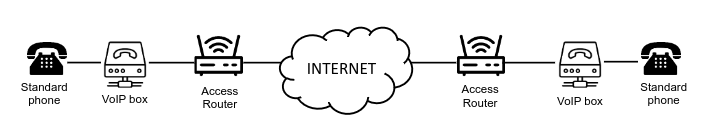
\includegraphics[width=0.8\textwidth]{pictures/6/adaptedVoip.png}
	\end{figure}
\end{itemize}
\subsection{VoIP-PTSN}
La comunicazione avviene tra un terminale VoIP e un terminale PTSN.
I pacchetti vocali vengono instradati usando internet solo in parte del cammino, mentre il resto del cammino utilizza la rete PTSN.
\begin{figure}[H]
	\centering
	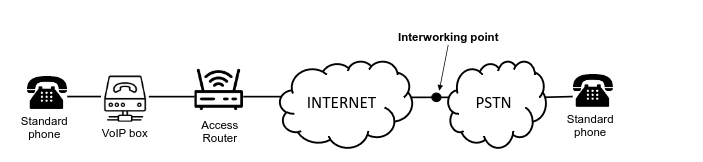
\includegraphics[width=0.8\textwidth]{pictures/6/voipptsn.png}
\end{figure}
\subsection{VoIP-Mobile Radio Network}
La comunicazione avviene tra un terminale VoIP e un terminale mobile.
Deve essere garantita l'interconnessione tra la rete internet e la rete mobile, che può essere 3G, 4G o 5G (vedremo più avanti).
\begin{figure}[H]
	\centering
	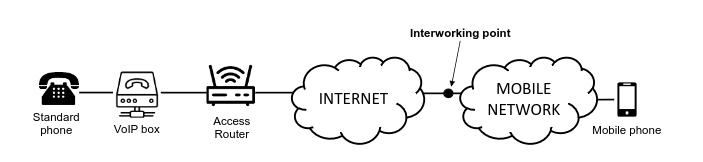
\includegraphics[width=0.8\textwidth]{pictures/6/voipmobile.png}
\end{figure}
\section{Motivazioni dell'adozione del VoIP}
Una integrazione standardizzata tra IP e la rete telefonica presenta un'opportunità per realizzare un sistema di comunicazione globale.
L'unica rete per i dati universale è la rete IP, e quindi è naturale che la telefonia si evolva verso l'uso di IP.
Questa integrazione offre benefizi sia per i consumatori che per i fornitori di servizi, tra cui:
\begin{itemize}
	\item \textbf{Per gli operatori}:
	\begin{itemize}
		\item Unificazione dei sistemi di controllo e gestione.
		\item Facilità di implementazione di nuovi servizi relativi alla voce su reti IP.
		\item Riduzione dei costi operativi.
	\end{itemize}
	\item \textbf{Per i consumatori}:
	\begin{itemize}
		\item Adozione di dispositivi smart che permettono di utilizzare servizi aggiuntivi facilmente configurabili (e.g. forwarding delle chiamate).
		\item Disaccoppiamento dell'identità dell'utente dall'indirizzo IP associato al terminale di linea.
		Questo permette di utilizzare lo stesso numero di telefono su più dispositivi, o di effettuare chiamate a prescindere dalla posizione geografica.
		\item Integrazione di comunicazione multimediale.
		\item Regolazione della qualità del servizio.
	\end{itemize}
\end{itemize}
\section{Codifica vocale}
La codifica permette di rappresentare digitalmente un segnale audio, quindi permette di trasformarlo in uno stream di bit.
La componente vocale ha una banda massima di circa $20\text{kHz}$, ma la maggior parte dell'informazione utile si trova nei primi $4\text{kHz}$.
Una codifica può avere diversi livelli di fedeltà, e quindi può essere più o meno compressa.
Vediamo ora diversi tipi di codificatori.
\subsection{Codifiche a onda}
Permettono di codificare un segnale con banda $\mathcal{B}$ senza perdite (a meno dell'errore di quantizzazione).
Le operazioni da effettuare sono 
\begin{itemize}
	\item \textbf{Campionamento}: si campiona il segnale a una frequenza $f_s$ che deve essere almeno $2\mathcal{B}$ (teorema di Nyquist).
	\item \textbf{Quantizzazione}: si quantizza il segnale campionato, associando a ogni campione un numero. Questa operazioni è irreversibile e introduce un errore di quantizzazione.
	La quantizzazione può essere uniforme o non uniforme.
\end{itemize}
\subsubsection{Pulse Code Modulation (PCM)}
Considera $\mathcal{B}=4\text{kHz}$, quindi $f_s=8\text{kHz}$.
Si quantizzano i campioni con $8$ bit, quindi si ottiene un bitrate di $64\text{kbit/s}$.
Viene adottata una quantizzazione non uniforme, che permette di ridurre l'errore di quantizzazione per i segnali a bassa ampiezza.
Questo tipo di quantizzazione è particolarmente adatto alle dinamiche percepite dall'orecchio umano.
\subsubsection{Differential PCM (DPCM)}
Campioni vicini nel tempo sono correlati, quindi è conveniente utilizzare metodi predittivi per stimare il valore del campione successivo a partire dal campione precedente.
Viene quindi codificata la differenza tra il campione attuale e quello precedente, invece del campione stesso.
Grazie alla correlazione, la varianza della differenza è minore della varianza dei campioni, 
quindi è possibile utilizzare meno bit per quantizzare la differenza, riducendo il bitrate.
\subsubsection{Adaptive DPCM (ADPCM)}
Le prestazioni migliorano con una quantizzazione adattiva e non lineare, quindi adattiamo la quantizzazione in base a i trend del segnale.
\subsection{Codec vocali}
Con queste tecnologie vengono usati modelli per riprodurre la voce umana in base alle sue caratteristiche intrinseche, allo scopo di rimuovere le ridondanze.
Questo tipo di codifica porta ad avere un ottima efficienza, ma è complessa e introduce ritardi elevati. Inoltre, è particolarmente sensibile a rumori di fondo.
Il tipo più popolare è il \textbf{linear vocoder} (LPC).

\bigskip
La voce è composta da due tipi di suoni:
\begin{itemize}
	\item \textbf{Voiced}: tipici delle vocali, caratterizzati da un suono periodico, con una certa frequenza fondamentale (pitch).
	\item \textbf{Unvoiced}: tipici delle consonanti, caratterizzati da un suono aperiodico, con una frequenza fondamentale molto alta.
\end{itemize}
Il processo biologico di produzione della voce umana è composto da tre fasi:
\begin{enumerate}
	\item Produzione del respiro (l'aria viene espulsa dai polmoni).
	\item Generazione del suono (le corde vocali vibrano)
	\item Modulazione del suono (viene dato il tratto vocal)
\end{enumerate}
Questo processo viene modellato attraverso un modello fonemico (fonema = unità del suono), definendo un filtro di riverberazione.
\begin{figure}[H]
	\centering
	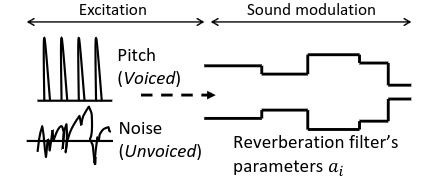
\includegraphics[width=0.8\textwidth]{pictures/6/Phoneme.png}
\end{figure}
Nella fase di eccitazione consideriamo la produzione del respiro e la generazione del suono, che vengono modellati come un segnale di eccitazione.
Il segnale generato è un treno di impulsi con un certo tono, o rumore bianco, a seconda che il suono sia voiced o unvoiced.
La modulazione del suono è modellata attraverso un filtro di riverberazione con parametri $a_i$, che rappresenta il tratto vocale.
\subsubsection{LPC-analisi}
A intervalli regolari (10-20 ms) vengono stimati i parametri per il fonema $s(n)$, vengono quantizzati e trasmessi.
\begin{itemize}
	\item Voiced ($\mathcal{V}$)/Unvoiced ($\mathcal{U}$) flag.
	\item Periodo di pitch $P$ (se voiced) o varianza del rumore (se unvoiced) del segnale di eccitazione $s'(n)$.
	\item Coefficienti lineari del filtro di riverberazione $a_i$.
	\item Gain $G$ del filtro di riverberazione.
\end{itemize}
Il segnale ottenuto è $s'(n)=G\sum_{i=1}^M a_i s'(n-i)$.
I parametri vengono scelti in modo da minimizzare la funzione d'errore $e(n)=|s(n)-s'(n)|$
\begin{figure}[H]
	\centering
	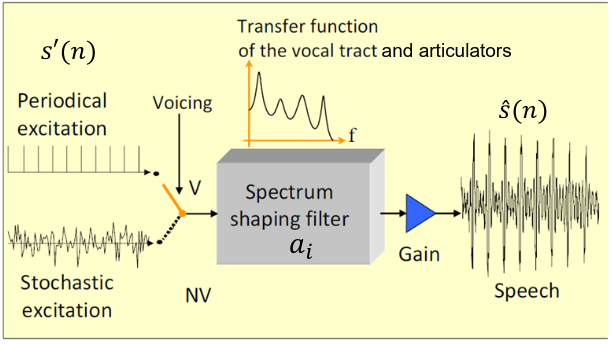
\includegraphics[width=0.8\textwidth]{pictures/6/lpcanalisi.png}
	\caption{Analisi in LPC}
\end{figure}
\subsubsection{LPC-sintesi}
Nella fase di decodifica un sintetizzatore ricostruisce il segnale vocale a partire dai parametri ricevuti.
\begin{figure}[H]
	\centering
	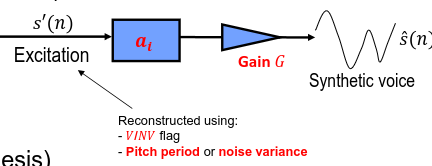
\includegraphics[width=0.8\textwidth]{pictures/6/lpcsintesi.png}
	\caption{Sintesi in LPC}
\end{figure}
Lo svantaggio di questo tipo di codifica è che introduce molto ritardo, a causa della complessità del processo di analisi e sintesi.
Inoltre, la voce ricostruita è comprensibile ma non è naturale, e il sistema è molto sensibile a rumori di fondo.
Però, è molto efficiente, e permette di raggiungere bitrate molto bassi (fino a 2.4 kbit/s).
\section{Codec ibridi}
I codec ibridi usano le tecniche dei vocoder lineari, ma ottimizzano alcuni aspetti.
Vediamo alcuni esempi:
\begin{itemize}
	\item \textbf{MultiPulse-Excited Linear Prediction (MPELP)}: Composto da $N$ impulsi equidistanti con ampiezza variabile. Non c'è distinzione tra suoni voiced e unvoiced.
	La posizione e ampiezza degli impulsi è determinata in modo da diminuire l'errore di quantizzazione.
	\item \textbf{GSM encoder (RPE-LTP)}: I vari bit codificati appartengono a diversi livelli di protezione (massimo, medio e nessuno).
	\item \textbf{Code Excited Linear Prediction (CELP)}: Le sequenze di eccitazioni vengono prese da un codice di eccitazione, che è un insieme di sequenze predefinite.
	La sequenza di eccitazione da utilizzare è quella che minimizza l'errore di quantizzazione. La ricerca della sequenza rallenta molto il processo, ma è possibile ottimizzare la ricerca.
\end{itemize}
\subsection{Misure di qualità}
La metrica principale per misurare la qualità di un codec è il MOS (Mean Opinion Score), che è una misura soggettiva della qualità percepita da un gruppo di ascoltatori.
È una scala da 1 a 5, dove 1 è la qualità più bassa e 5 è la qualità più alta.
Questo metodo è complesso e costoso da implementare.
\begin{figure}[H]
	\centering
	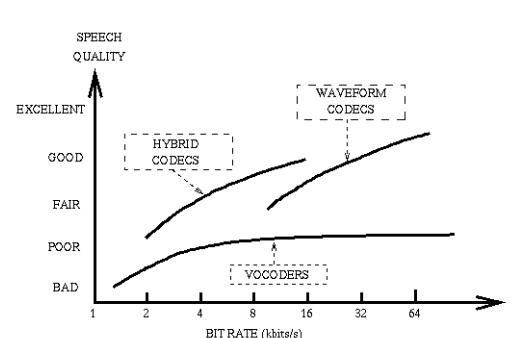
\includegraphics[width=0.5\textwidth]{pictures/6/mos.png}
	\caption{Scala MOS dei codec vocali}
\end{figure}
\section{Degradazione vocale}
Oltre alla qualità del codec, la qualità della voce può essere degradata da altri fattori, tra cui:
\begin{itemize}
	\item ritardo 
	\item perdita totale o parziale di segmenti vocali
\end{itemize}
Il ritardo può essere causato da diversi fattori
\begin{figure}[h]
	\centering
	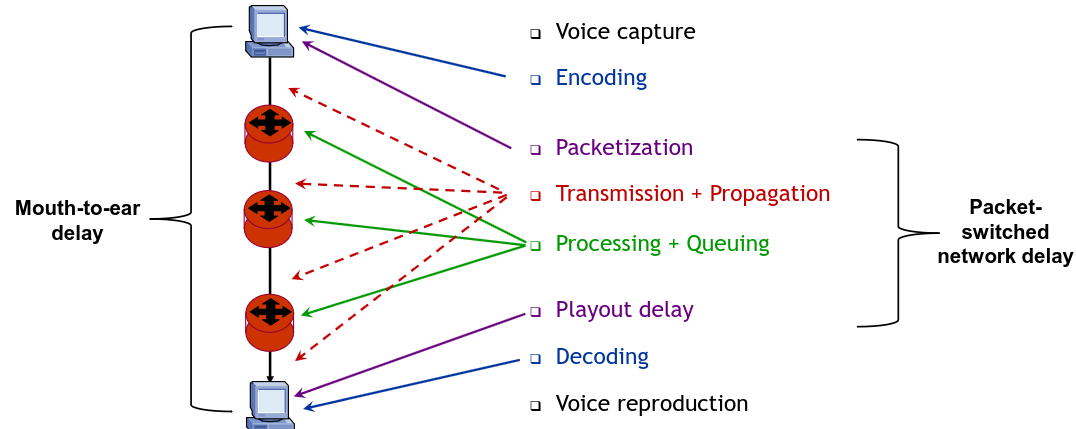
\includegraphics[width=0.8\textwidth]{pictures/6/delay.png}
	\caption{Processi della comunicazione con VoIP}
\end{figure}
\subsection{Ritardi da pacchettizzazione}
In questa procedura uno o più segmenti vocali vengono raggruppati per la trasmissione su una rete a commutazione di pacchetto.
In questo modo, si evita di inviare pacchetti con pochi dati, ma si introduce un ritardo di pacchettizzazione, che è il tempo necessario per raggruppare i segmenti vocali.
Il ritardo dipende dalla lunghezza dei segmenti e dal loro numero.
\begin{figure}[H]
	\centering
	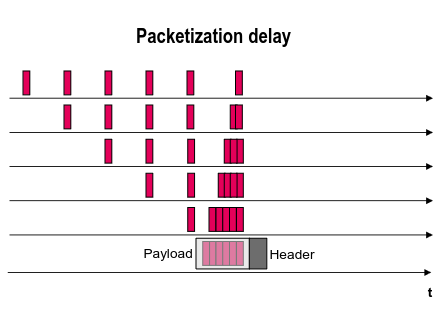
\includegraphics[width=0.5\textwidth]{pictures/6/packetization.png}
	\caption{Ritardo da pacchettizzazione}
\end{figure}
\subsection{Ritardi da trasmissione e propagazione}
\begin{figure}[H]
	\centering
	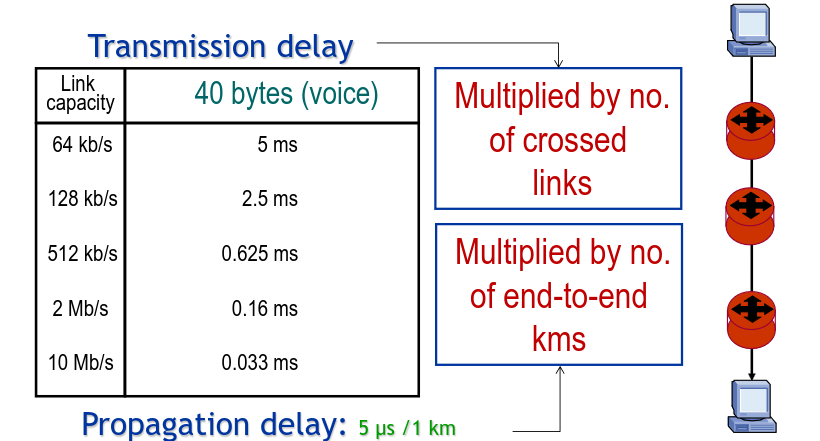
\includegraphics[width=0.5\textwidth]{pictures/6/transmission_propagation.png}
	\caption{Ritardo da trasmissione e propagazione}
\end{figure}
\subsection{Ritardo di elaborazione}
Il dispositivo di elaborazione dei pacchetti (switch, router, ecc\dots) introduce un ritardo di elaborazione.
Questo ritardo è dato dall'attraverso del piano dati (lookup tabelle e operazioni sui pacchetti).
Tendenzialmente è trascurabile, se i router e switch sono ben progettati sono nell'ordine di microsecondi.
\subsection{Ritardo di queuing}
\begin{figure}[H]
	\centering
	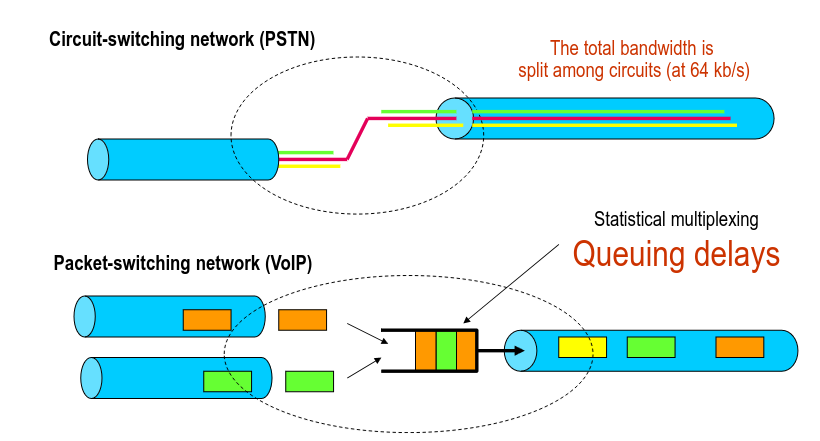
\includegraphics[width=0.8\textwidth]{pictures/6/queuing.png}
	\caption{Ritardo di queuing}
\end{figure}
\subsection{Ritardo per il playout e compensazione del jitter}
Il jitter è la variazione tra i ritardi di arrivo dei pacchetti vocali, rispetto alla spaziatura temporale alla sorgente.
\begin{figure}[H]
	\centering
	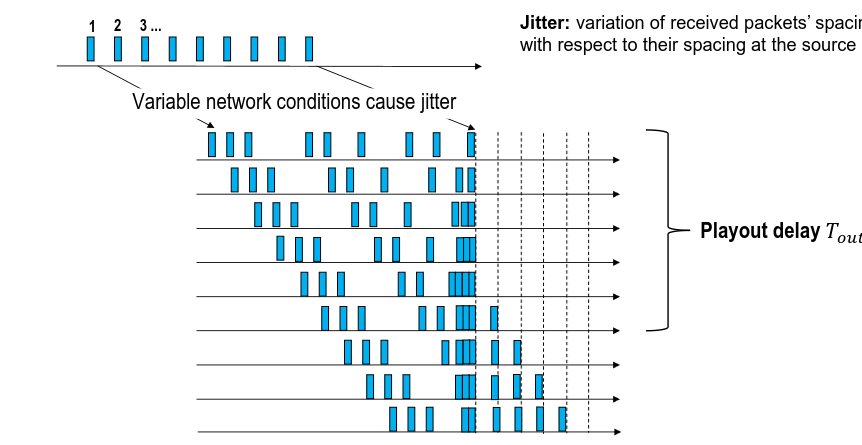
\includegraphics[width=0.8\textwidth]{pictures/6/jitter.png}
	\caption{Ritardo per il playout e compensazione del jitter}
\end{figure}\noindent
I pacchetti vengono memorizzati in una coda di playout.
Il primo pacchetto deve essere riprodotto dal ricevitore dopo un certo ritardo che compensa il jitter (playout delay $\text{T}_\text{out}$).
Può essere fisso o adattivo in base alle condizioni della rete.
\subsection{Soppressione del silenzio}
Nelle conversazioni duplex il canale viene usato mediamente per il $50\%$ del tempo.
Inoltre, le interruzioni vocali (ad esempio, quando una persona sta pensando a cosa dire) possono essere frequenti.
Nelle reti a commutazione di pacchetto viene adottata la soppressione del silenzio, in modo da ridurre la banda occupata.
Il silenzio va soppresso senza dare la sensazione che sia caduto il collegamento, quindi viene introdotto del rumore.
Per determinare se un segmento vocale è silenzioso o meno, viene utilizzato un algoritmo di rilevamento del silenzio, basato sui livelli di energia del segnale.
\section{VoIP signalling}
I protocolli si segnalazione controllano le chiamate, non sono direttamente coinvolti nella trasmissione dei dati vocali, ma sono responsabili di stabilire, gestire e terminare le chiamate.
Ci sono due tipi di segnalazione:
\begin{itemize}
	\item \textbf{In-band signalling}: usa lo stesso canale delle chiamate.
	\item \textbf{Out-of-band signalling}: usa un canale separato per la segnalazione.
\end{itemize}
\subsection{Signalling in reti PSTN}
Nelle reti PSTN, il signalling riguarda solo le chiamate e coinvolge:
\begin{itemize}
	\item \textbf{Il chiamante}: inizializzazione della chiamata.
	\item \textbf{La rete}: instradamento della chiamata e prenotazione delle risorse.
	\item \textbf{Il chiamato}: ricezione della chiamata.
\end{itemize}
In base allo scambio di messaggi di segnalazione, la rete effettua il controllo di accesso, controllo di ammissione di chiamata e carico di costi.
Il protocollo utilizzato è il \textbf{Signalling System No. 7 (SS7)}, basato su una rete a commutazione di pacchetto e ampiamente utilizzato nelle reti GSM.
\begin{figure}[H]
	\centering
	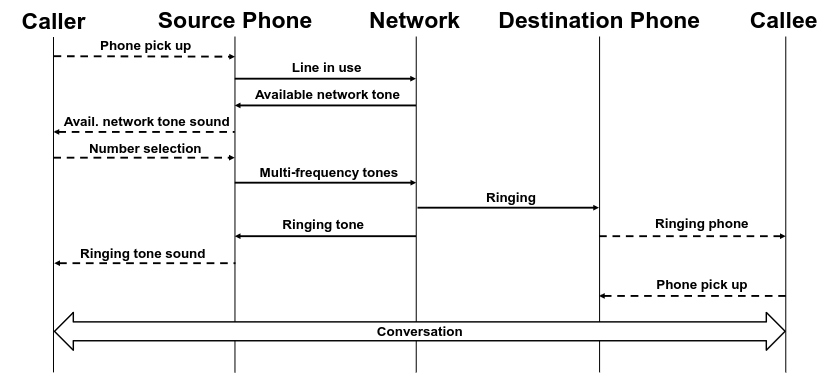
\includegraphics[width=0.8\textwidth]{pictures/6/ss7.png}
	\caption{Diagramma di sequenza di SS7}
\end{figure}
\subsection{Signalling in reti VoIP}
Nelle reti IP il signalling può essere ridotto in quanto il routing viene effettuato dal protocllo IP, semplicemente è necessario adottare un sistema simile a DNS per risolver i nomi dei terminali in indirizzi IP.
Quindi, è sufficiente implementare un protocollo per allerare il terminale chiamato, e per negoziare i parametri della chiamata (ad esempio, il codec da utilizzare).
In realtà, vengono adottare dei protocolli specifici per gestire meglio alcune funzionalità, come ad esempio il controllo di accesso, il controllo di ammissione di chiamata e il carico di costi.
Ci sono vari protocolli di segnalazione per VoIP, tra cui:
\begin{itemize}
	\item \textbf{Session Initiation Protocol (SIP)}
	\item \textbf{H.323}
\end{itemize}
SIP è il più utilizzato oggi giorno, quindi ci concentreremo su questo protocollo.
\section{Session Initiation Protocol (SIP)}
Protocollo creato nel 2002 per inizializzare chiamata e videochiamate.
Consente di effettuare chiamate tra utenti attraverso degli identificatori univoci (URI,  SIP Uniform Resource Identifier),
che sono simili agli indirizzi email (e.g. user@domain.tld).
Il campo user può essere numerico per essere compatibile con lo standard E.164 delle reti PSTN.
L'identificatore è relativo all'utente, non al terminale, dunque ha la possibilità di accedere al servizio da diversi terminali (personal mobility).
Questo richiede l'adozione di due meccanismi, registrazione e localizzazione.
L'identificatore può essere associato a più terminali contemporaneamente, inoltre è possibile associare più identificatori a uno stesso terminale.
SIP è un protocollo di livello applicativo client-server
Ogni nodo di rete che è coinvolto in SIP tendenzialmente implementa sia funzionalità di client che di server.
\subsection{Metodi e response codes}
Le richieste dei client vengono chiamate metodi, in totale sono 14, qui vediamo i più importanti:
\begin{table}[H]
	\begin{tabular}{l|l}
		\textbf{Metodo} & \textbf{Descrizione} \\ \hline
		\texttt{INVITE} & Inizia la chiamata invitando un utente. \\
		\texttt{ACK} & Conferma la creazione della connessione. \\
		\texttt{BYE} & Termine (o trasferimento) di una chiamata. \\
		\texttt{CANCEL} & Annulla una richiesta in sospeso. \\
		\texttt{REGISTER} & Registra presso un location server. \\
		\texttt{OPTIONS} & Richiede informazioni. \\
	\end{tabular}
\end{table}\noindent
In SIP non c'è garanzia di consegna dei messaggi, potrebbero quindi dover essere ritrasmessi.

\bigskip\noindent
Le risposte contengono un codice che descrive il risultato della richiesta che è stata processata dal server, e sono divise in 6 classi:
\begin{itemize}
	\item \textbf{1xx}: Informative, indicano che la richiesta è stata ricevuta e che il processo è in corso.
	\item \textbf{2xx}: Successo, indicano che la richiesta è stata processata con successo.
	\item \textbf{3xx}: Redirezione, indicano che è necessario un ulteriore passo per completare la richiesta.
	\item \textbf{4xx}: Errore del client, indicano che c'è stato un errore nella richiesta inviata dal client.
	\item \textbf{5xx}: Errore del server, indicano che c'è stato un errore nel server che ha processato la richiesta.
\end{itemize}
Le possibili risposte sono 75, qui vediamo le più importanti:
\begin{table}[H]
	\begin{tabular}{l|l|l|l|l|l}
		\textbf{Codice} & \textbf{Descrizione} & \textbf{Codice} & \textbf{Descrizione}  & \textbf{Codice} & \textbf{Descrizione}\\ \hline
		100 & continue & 400 & bad request & 500 & internal error\\
		180 & ringing & 401 & unauthorized & 501 & not implemented\\
		181 & forwarding & 403 & forbidden & 600 & busy\\
		182 & queuing & 404 & not found & 601 & decline\\
		200 & OK & 408 & request timeout & 604 & does not exist\\
		300 & multiple choices & 480 & unavailable & 606 & not acceptable\\
		301 & moved permanently & 481 & invalid Call ID & & \\
		302 & moved temporarily & 482 & loop detected & &
	\end{tabular}
\end{table}
\subsection{Transazioni}
Le richieste e le risposte vengono raggruppate in transazioni, con l'obiettivo di stabilire delle sessioni.
Una sessione è uno scambio attivo di messaggi multimediali e consiste di:
\begin{itemize}
	\item Una richiesta
	\item Una risposta informativa (1xx)
	\item Una risposta finale
\end{itemize}
I messaggi \texttt{INVITE} richiedono un \texttt{ACK} finale per confermare che la sessione è stata stabilita. Questo messaggio finale di conferma viene considerato come una nuova transazione, senza risposta.
\begin{figure}[H]
	\centering
	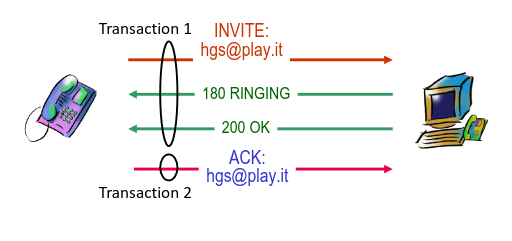
\includegraphics[width=0.6\textwidth]{pictures/6/session.png}
	\caption{Instaurazione di una sessione SIP}
\end{figure}
\subsection{Formati di richieste e risposte}
SIP è un protocollo character-oriented, come HTTP, quindi i messaggi sono composti da linee di testo.
Questo rende i messaggi facilmente leggibili.
\begin{figure}[H]
	\centering
	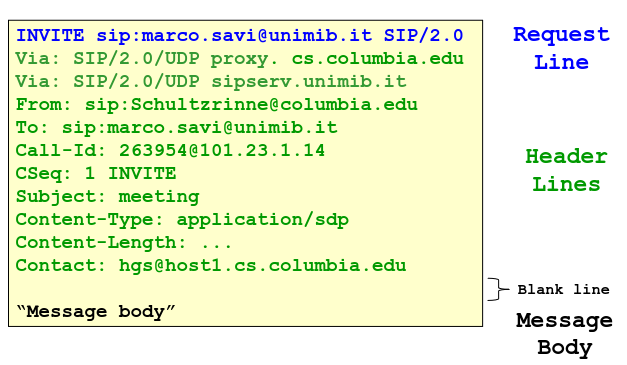
\includegraphics[width=0.8\textwidth]{pictures/6/siprequest.png}
	\caption{Formato di una richiesta SIP}
\end{figure}
\begin{figure}[H]
	\centering
	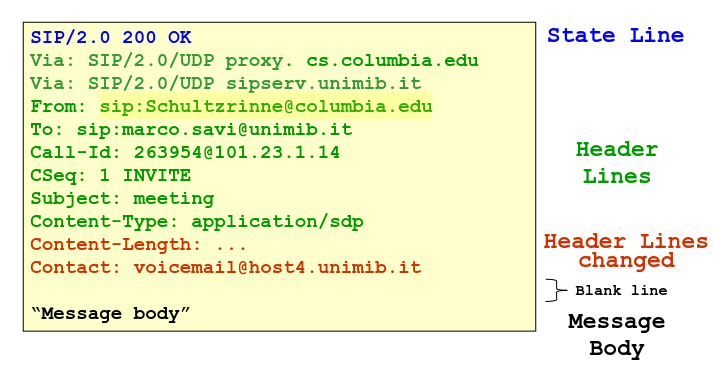
\includegraphics[width=0.8\textwidth]{pictures/6/sipresponse.png}
	\caption{Formato di una risposta SIP}
\end{figure}
Il formato dei campi dell'header sono del tipo \texttt{parametro:valore}.
\subsection{Elementi di rete}
La rete viene divisa in domini, ognuno di questi include gli elementi rappresentati in figura \ref{fig:elementiReteSIP}.
\begin{figure}[H]
	\centering
	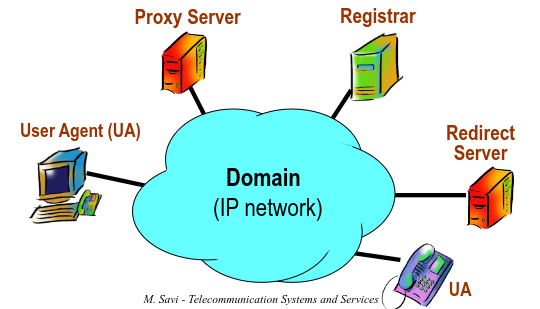
\includegraphics[width=0.8\textwidth]{pictures/6/elementiReteSIP.png}
	\caption{Elementi di rete SIP}
	\label{fig:elementiReteSIP}
\end{figure}
I server proxy si occupano di comunicare con la loro controparte negli altri domini.
\subsubsection{User Agent (UA)}
È il chiamante (UA client) o il chiamato (UA server) di una sessione che viene stabilita attraverso SIP.
\begin{figure}[H]
	\centering
	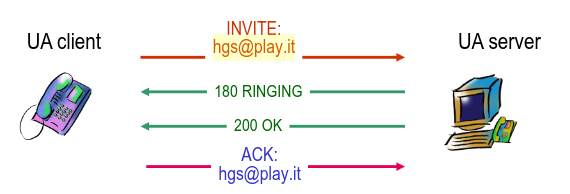
\includegraphics[width=0.7\textwidth]{pictures/6/UA.png}
	\caption{User Agent SIP}
\end{figure}
\subsubsection{Registrar}
In un dominio il registrar associa l'URI SIP di un utente con l'indirizzo del UA che lo rappresenta.
Per fare in modo che un utente sia raggiungibile attraverso uno specifico UA, l'utente si deve registrare presso il registrar.
Una richiesta di \texttt{REGISTER} viene inviata periodicamente.
\begin{figure}[H]
	\centering
	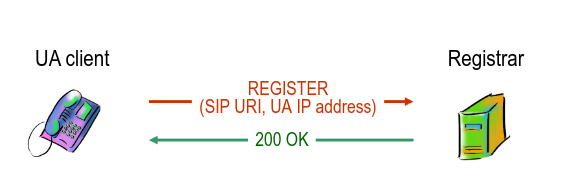
\includegraphics[width=0.7\textwidth]{pictures/6/registrar.png}
	\caption{Registrar SIP}
\end{figure}\noindent
Ci sono tre possibili modalità per ottenere l'indirizzo del Registrar per l'UA:
\begin{itemize}
	\item \textbf{Configurazione statica}
	\item \textbf{DNS}
	\item \textbf{Multicast}: la richiesta di \texttt{REGISTER} viene mandata in multicast all'indirizzo sip.mcast.net (224.0.1.75). 
\end{itemize}
\subsubsection{Proxy server}
Router a livello applicativo che si occupano di instradare le richieste SIP tra i domini.
\begin{figure}[H]
	\centering
	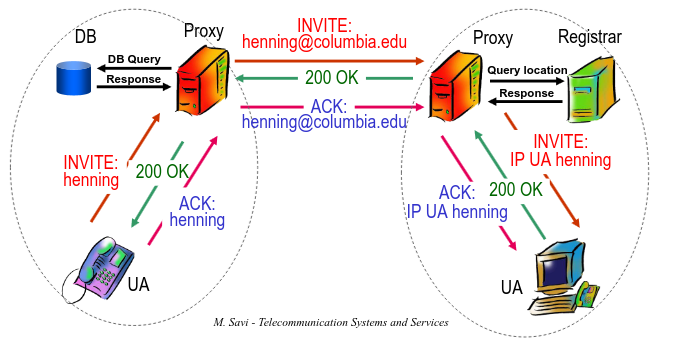
\includegraphics[width=0.7\textwidth]{pictures/6/proxy.png}
	\caption{Proxy server SIP}
\end{figure}
\subsubsection{Redirect server}
Riceve le richieste SIP e risponde con un messaggio di redirezione, indicando al client di inviare la richiesta a un altro server.
Tipicamente vengono implementati direttamente negli UA.
\begin{figure}[H]
	\centering
	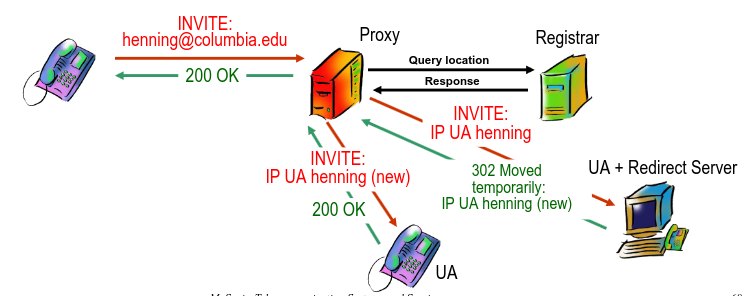
\includegraphics[width=0.7\textwidth]{pictures/6/redirect.png}
	\caption{Redirect server SIP}
\end{figure}
\subsubsection{SIP forking}
Un server proxy che riceve una richiesta da un client può inoltrarla a più destinazioni (automatic call distribution).
Questo succede quando un utente è registrato su più UA. Questa operazione può avvenire in modo seriale o parallelo.
Nel caso di distribuzione parallela, la prima risposta positiva che arriva viene mantenuta, e le altre se necessario vengono cancellate.
\subsection{Session Description Protocol}
Questo protocollo viene utilizzato per descrivere i parametri della sessione. 
I messaggi SDP vengono trasportati in modo trasparente come body dei messaggi SIP.
Tipicamente, il messaggio \texttt{INVITE} contiene un messaggio SDP che descrive i parametri della sessione che il chiamante vuole stabilire, 
e la risposta \texttt{200 OK} contiene un messaggio SDP che descrive i parametri della sessione che il chiamato accetta.
Se il client non ha incluso il body SDP nell'\texttt{INVITE}, lo deve necessariamente fare nel \texttt{ACK} finale.
\begin{figure}[H]
	\centering
	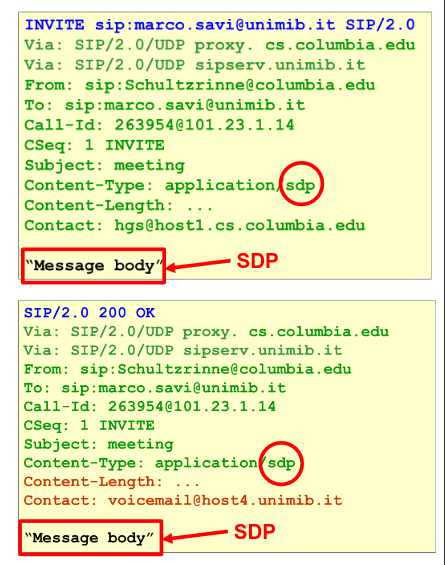
\includegraphics[width=0.5\textwidth]{pictures/6/sdp.png}
	\caption{Scambio di messaggi SIP con body SDP}
\end{figure}
Il body di un messaggio SDP contiene diversi campi, tra cui:
\begin{itemize}
	\item Nome e scopo della sessione
	\item Durata della sessione
	\item Media da trasmettere (audio, video, ecc\dots)
	\item Informazioni per supportare tali media
	\item Informazioni sul contatto
\end{itemize}
I campi sono rappresentati in modo simile a quelli di un messaggio SIP, con la sintassi \texttt{parametro=valore}.
\begin{figure}[H]
	\centering
	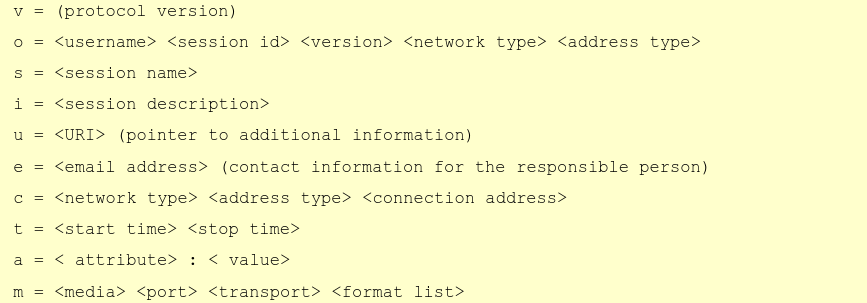
\includegraphics[width=0.8\textwidth]{pictures/6/parameters.png}
	\caption{Esempio di body SDP}
\end{figure}
\subsection{Instradamento delle risposte}
SIP assicura the le risposte seguano lo stesso percorso delle richieste, attraverso il campo \texttt{Via} dell'header.
Questo campo identifica i Proxy server che hanno instradato la richiesta, e viene aggiornato ogni volta che la richiesta attraversa un nuovo Proxy server.
Viene aggiunto da ogni Proxy server, in testa all'header, un nuovo campo \texttt{Via} con il proprio indirizzo.
In questo modo, quando il server risponde, può seguire il percorso inverso, rimuovendo i campi \texttt{Via} man mano che attraversa i Proxy server.
\begin{figure}[H]
	\centering
	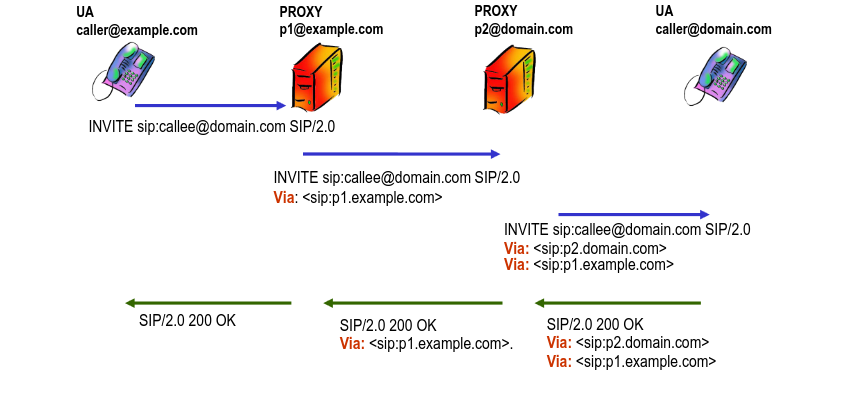
\includegraphics[width=0.8\textwidth]{pictures/6/response.png}
	\caption{Instradamento delle risposte SIP}
\end{figure}
Vengono utilizzati due meccanismi per assicurare che richieste adiacenti seguano lo stesso percorso:
\begin{itemize}
	\item \textbf{Route recording}: attraverso il campo \texttt{Record-Route}.
	\item \textbf{Source-based routing}: attraverso il campo \texttt{Route}.
\end{itemize}
\begin{figure}[H]
	\centering
	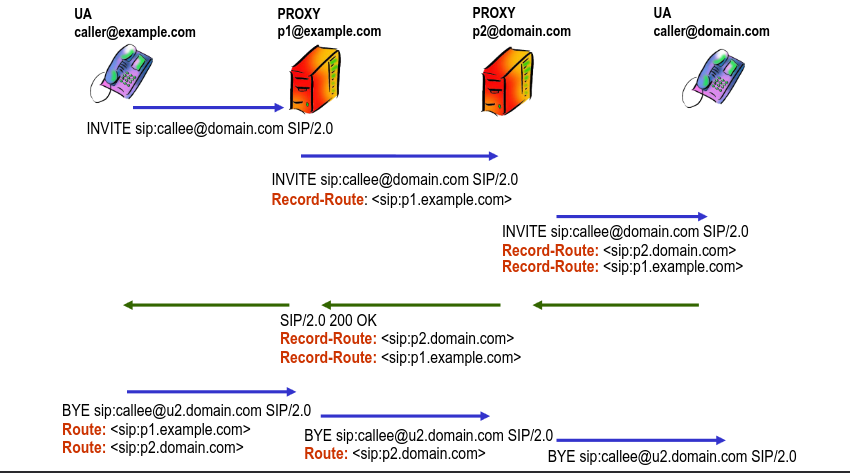
\includegraphics[width=0.8\textwidth]{pictures/6/routing.png}
	\caption{Instradamento delle richieste SIP}
\end{figure}
\subsection{Ulteriori metodi}
Possono essere utilizzati per sospendere, modificare o riattivare il setup di una chiamata quando devono essere effettuate delle azioni prima che possa essere completato.
\subsubsection{PRACK}
Provisional ascknowledgement, quando un server dopo aver ricevuto una richiesta manda una risposta conclusiva (2xx), dopodiché aspetta un ACK dal client.
Se l'ACK non arriva, la riposta 2xx viene ritrasmessa. Se l'ACK non viene mandato perché il client deve effettuare altre operazioni, allora viene usato il PRACK.
\begin{figure}[H]
	\centering
	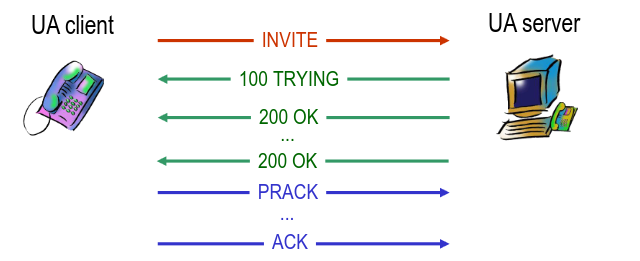
\includegraphics[width=0.8\textwidth]{pictures/6/prack.png}
	\caption{Utilizzo del metodo PRACK}
\end{figure}
\subsubsection{UPDATE}
Una volta che il setup è concluso, un INVITE viene rimandato, per due motivi:
\begin{itemize}
	\item Cambiare sessione SIP
	\item Modificare i media SDP
\end{itemize}
Se solamente i media SDP devono essere modificati, è possibile utilizzare il metodo UPDATE, che non richiede una nuova sessione SIP.
Gli UPDATE possono anche essere usati durante il setup.
\begin{figure}[H]
	\centering
	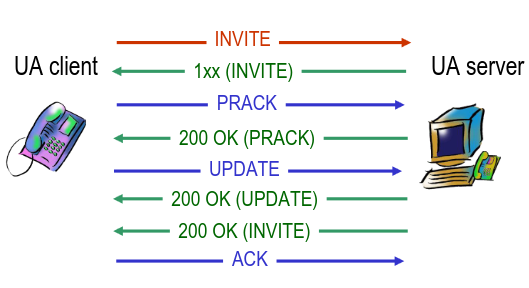
\includegraphics[width=0.8\textwidth]{pictures/6/update.png}
	\caption{Utilizzo del metodo UPDATE}
\end{figure}
\bigskip\noindent
Inoltre ci sono altri metodi.
\subsubsection{REFER}
Indica che il chiamante deve contattare una terza parte, indicata dal campo \texttt{Refer-to}, può essere usato per trasferire una chiamata a un altro utente.
\begin{figure}[H]
	\centering
	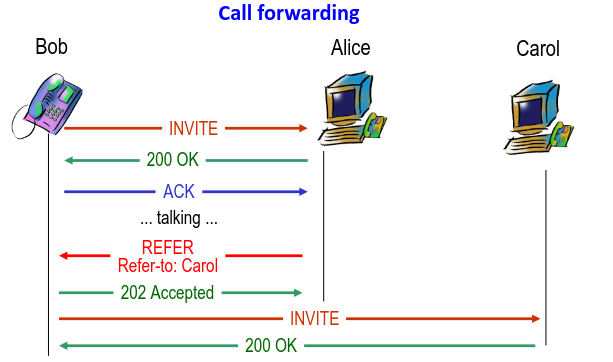
\includegraphics[width=0.8\textwidth]{pictures/6/refer.png}
	\caption{Utilizzo del metodo REFER}
\end{figure}
\subsubsection{NOTIFY}
Utilizzato per implementare servizi di notifica, ad esempio una volta che una REFER è stata accettata, il server può inviare una NOTIFY all'utente che ha inviato la REFER, per informarlo dell'esito della richiesta.
\begin{figure}[H]
	\centering
	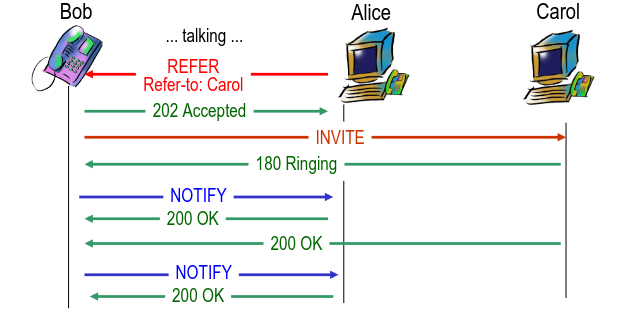
\includegraphics[width=0.8\textwidth]{pictures/6/notify.png}
	\caption{Utilizzo del metodo NOTIFY}
\end{figure}